% ----------------------------------------------------------
% Proposta
% ----------------------------------------------------------
\chapter{Proposta de projeto}
\label{chp:proposta}

\section{Métodos de pesquisa}
\label{sec:métodos}

A presente proposta está planejada para ser executada em 3 fases.
%
A primeira fase tem por objetivo encontrar uma forma de relacionar a evidência coletada de um contêiner a sua origem de forma que o processo seja reprodutível. 
%
Para atingir este objetivo será implementado um protótipo de coleta de memória de uma máquina virtual executando contêiners em um notebook.
%
A segunda fase tem por objetivo encontrar uma forma de transportar a evidência coletada a um local de armazenamento garantindo a cadeia de custódia.
%
Para atingir este objetivo, será definida uma cadeia de custódia. De posse desta será realizada em uma nuvem computacional e envolverá o transporte da evidência para uma máquina física fora da nuvem.
%
A terceira parte tem por objetivo a realização da análise de alguma vulnerabilidade utilizando-se do material coletado na primeira fase do projeto.
%
As ações para se atingir este objetivo serão realizadas em um notebook com ferramental voltado a análise forense em memória.

\section{O que foi feito e cronograma esperado para os próximos passos}
\label{sec:até_agora}

Até então foram realizados com sucesso a duas primeiras partes do projeto.

%
Parte 1: A associação da evidência de memória coletada do contêiner de uma máquina virtual foi associada a sua origem através do \textit{hash} de identificação da imagem do contêiner. O processo de coleta foi reproduzido com sucesso diversas vezes.
%
Parte 2: O transporte da evidência para uma máquina física fora da nuvem utilizando camada de transporte seguro a assinatura da mensagem.
%

Para o restante do projeto, que consiste da parte 3, espera-se seguir o cronograma descrito na figura 12 onde serão executadas as seguintes atividades.

\begin{itemize}
 \item \textbf{Estudo das ferramentas de análise de memória}: Onde serão avaliadas ferramentas de análise de memória na busca por alguma que consiga decodificar as informações coletadas 
 \item \textbf{Implemenação / seleção de uma ferramenta de análise}: Nesta atividade será selecionada uma das ferramentas estudadas na atividade anterior. Caso nenhuma se mostre adequada, será implementada uma ferramente para o propósito da fase 3
 \item \textbf{Realização de análises com a ferramenta escolhida / criada}: Nesta fase ocorrerá a tentativa de analisar um malware encontrado em alguma coleta realizada na fase 1
\end{itemize}

\begin{figure}[htb!]
\footnotesize
\caption{Cronograma de projeto}
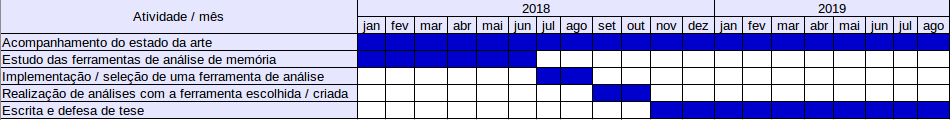
\includegraphics[scale=0.50]{crono-image.png}
\centering
\label{fig:cronograma}
\end{figure}

\section{Limitações}
\label{sec:limitacoes}

Como a solução descrita tem como foco coletar informações de memória no espaço do usuário (\textit{user space}), ela não consegue acessar o espaço de kernel (\textit{kernel space}). 
%
Assim, \fancyname em princípio não provê suporte a técnicas de investigação de malware que se baseiam em informações do \textit{kernel space}, como, por exemplo, a comparação de informações do bloco do ambiente do processo (\textit{Process Environment Block -- PEB}), que ficam no \textit{user space}, com informações do descritor de endereços de memória virtual (\textit{Virtual Address Descriptor -- VAD}), que fica no \textit{kernel space}. 
%
Análise de ameaças que realizam manipulação direta dos objetos do kernel (D.K.O.M.-- \textit{Direct Kernel Object Manipulation}) também não se beneficiam com a solução aqui proposta. 

\section{Contribuições}
\label{sec:contribuições}

A contribuição esperada da presente proposta é o de demonstrar que é possível coletar evidências de uma infra-estrutura em núvem de modo a atender os pré-requisitos de não violação de privacidade, não violação da jurisdição, reprodutibilidade do processo de coleta da evidência e garantia da cadeia de custódia.
%
Demonstrar que é possível realizar a análise de evidência de memória com apenas a parte \textit{user space} da memória coletada

